\documentclass[a4paper, papersize, titlepage]{jsarticle}
\usepackage[]{multicol} % 途中からtwocolumun \begin{multicols}{n}
\usepackage[dvipdfmx]{graphicx}

% for \mathbb{}, \begin{cases}
\usepackage{amsmath, amssymb}
\usepackage{type1cm} 
\usepackage{url}
\usepackage{comment}
\usepackage{mathtools} % for \coloneqq
\usepackage{eqnarray} % 連続するn式
\usepackage{here}


\usepackage{listings,jlisting} % 日本語のコメントアウトをする場合jlistingが必要
% ここからソースコードの表示に関する設定
\lstset{
  basicstyle={\ttfamily},
  identifierstyle={\small},
  commentstyle={\smallitshape},
  keywordstyle={\small\bfseries},
  ndkeywordstyle={\small},
  stringstyle={\small\ttfamily},
  frame={tb},
  breaklines=true,
  columns=[l]{fullflexible},
  numbers=left,
  xrightmargin=0zw,
  xleftmargin=3zw,
  numberstyle={\scriptsize},
  stepnumber=1,
  numbersep=1zw,
  lineskip=-0.5ex
}
% ここまでソースコードの表示に関する設定
% \begin{lstlisting}[caption=hoge,label=fuga] を用いる
% キャプション名「ソースコードn」を「プログラムn」に変えるには,\begin{document}の前に\renewcommand{\lstlistingname}{プログラム}
% https://qiita.com/ta_b0_/items/2619d5927492edbb5b03

% for hyperref
\usepackage[dvipdfmx, bookmarkstype=toc, colorlinks=false, pdfborder={0 0 0}, bookmarks=true, bookmarksnumbered=true]{hyperref}
\usepackage{pxjahyper}

\def\bm#1{\mbox{\boldmath $#1$}} % for bm (vector)

%%%%%%%%%%%%%%%%%%%%%%%%%%%%%%%%%%%%%%%%%%%%%%%%%%%%%%%%%%%%%%%%%%%%%%%%%%%%%%%%

\title{高度情報演習2C \\
【前半】テーマ1(真鍋)2回目レポート \\
~\\
ボタンUI内外のカーソル速さ調節による \\
ポインティング時間の短縮手法の提案
}
\author{片岡 凪 \thanks{芝浦工業大学 工学部 情報工学科 3年 学籍番号AL18036}}
\date{提出締切 2020年10月22日 \\
提出日 2020年10月21日}

\begin{document}

\maketitle
\setcounter{tocdepth}{3}
\tableofcontents

\newpage
\abstract{
Windows OSやMac OSで広く用いられているマウスカーソルの動作を改良し,ポインティング時間の短縮を図る.そのため,UI中のボタンの内外でカーソルの速さを調節する手法を提案し,その有効性を検証する.
}

\begin{multicols}{2}

\begin{comment}
・課題,解決策,手法の有効性の説明
・従来手法,提案手法
\end{comment}

%%%%%%%%%%%%%%%%%%%%%%%%%%%%%%%%%%%%%%%%%%%%%%%%%%%%%%%%%%%%%%%%%%%%%%%%%%%%%%%%

\section{従来手法の課題点}
2020年現在に広く用いられているマウスカーソルで高速なポインティングを試みると,よりカーソルの初期座標から離れたボタンほど,より高頻度で過剰にカーソルを進めてしまいやすい傾向が観測された~\cite{report_1}.過剰にカーソルを進めてしまうと,行き過ぎた距離差分を修正するためのタイムロスや,ポインティング位置のエラーが生じやすい.

一方,初期座標からある程度近いボタンに向けて高速なポインティングを試みた場合,1度の試行で目標のボタンに到達せず,足りない距離差分を修正しようとする傾向が観測された~\cite{report_1}.この場合も,修正のタイムロスやポインティング位置のエラーが生じやすいと考える.

%%%%%%%%%%%%%%%%%%%%%%%%%%%%%%%%%%%%%%%%%%%%%%%%%%%%%%%%%%%%%%%%%%%%%%%%%%%%%%%%

\section{提案手法}
本研究では上述の課題を踏まえ,カーソルがボタンの外側に位置するときはカーソルを速く,内側に位置するときはカーソルを遅くしてポインティングを時間を短縮する手法を提案する.

この手法によって,カーソルをボタンまで止めることなく高速に移動させ,行き過ぎることなくボタン内で停止させることが容易になると考える.位置修正の頻度が少なくなるため,それに伴うタイムロスとポインティング位置のエラーを低減させる効果が期待できる.

%%%%%%%%%%%%%%%%%%%%%%%%%%%%%%%%%%%%%%%%%%%%%%%%%%%%%%%%%%%%%%%%%%%%%%%%%%%%%%%%

\section{実験}

\subsection{検証内容}
以下の3つの手法のカーソルを実装したのち,それぞれの手法についてポインティングの時間と精度を測定,比較し,提案手法の有効性を検証する.
\begin{description}
\item[従来手法$X_0$.] ~\\ 速さを調節しない従来のカーソル
\item[提案手法$X_1$.] ~\\ ボタン外では従来通りに,ボタン内では低速に動作するカーソル
\item[提案手法$X_2$.] ~\\ ボタン外では高速に,ボタン内では低速に動作するカーソル
\end{description}

高速化がかえってポインティング時間を長くしてしまう可能性を考慮し,2つの提案手法$X_1, X_2$を実装と検証を行う.なお,ここに記載していない「ボタン外では高速に,ボタン内では従来通りに動作するカーソル」は,カーソルが制御できずに行き過ぎてしまいやすくなる結果が明白であるので除外している.

%%%%%%%%%%%%%%%%%%%%%%%%%

\subsection{実験器具}

以下の実験器具を用いて実験を行った.なお,器具の違いによる結果の差の発生を抑制するため,すべての被験者に同一の器具を使用させた.

\begin{itemize}
\item パーソナルコンピュータ
\item 24インチ外部モニター
\item 光学マウス
\item Unity \footnote{自作カーソルの実装に使用したゲームエンジン}
\item Microsoft Excel \footnote{作図に使用}
\item IBM SPSS Statistics \footnote{検定に使用}
\end{itemize}

%%%%%%%%%%%%%%%%%%%%%%%%%%%%%%%%%%%%%%%%%%%%%%%%%%%%%%%%%%%%%%%%%%%%%%%%%%%%%%%%

\subsection{実装}

\subsubsection{ボタンの実装}
ポインティング時間の測定のため,以下の図~\ref{button}のようにボタンを配置した.

ポインティング時間は,中央のボタンをポインティングする時刻と外側のアクティブなボタンをポインティングする時刻との差として定義し,測定した.アクティブなボタンは,1セットのポインティングをする度に,外側の8個のボタンからランダムに1つ選出される.3つの各手法それぞれについて, $8 \times 2 = 16$ セットの測定を行った.

1セット目のポインティングはそれ以降の試行とは慣れの度合が異なるものと考え,16セットの測定とは別にダミーの試行を行わせた.

中央のボタンと外側のボタンとの距離は,ポインティング時に「距離が足りなくなるケース」と「行き過ぎてしまうケース」の両方が観測されたものを採用した.

また,被験者の負担にならない範囲でより一般のポインティングを考えるため,ポインティングが均等な8方向になるようにボタンを配置している.

\begin{figure}[H]
 \centering
   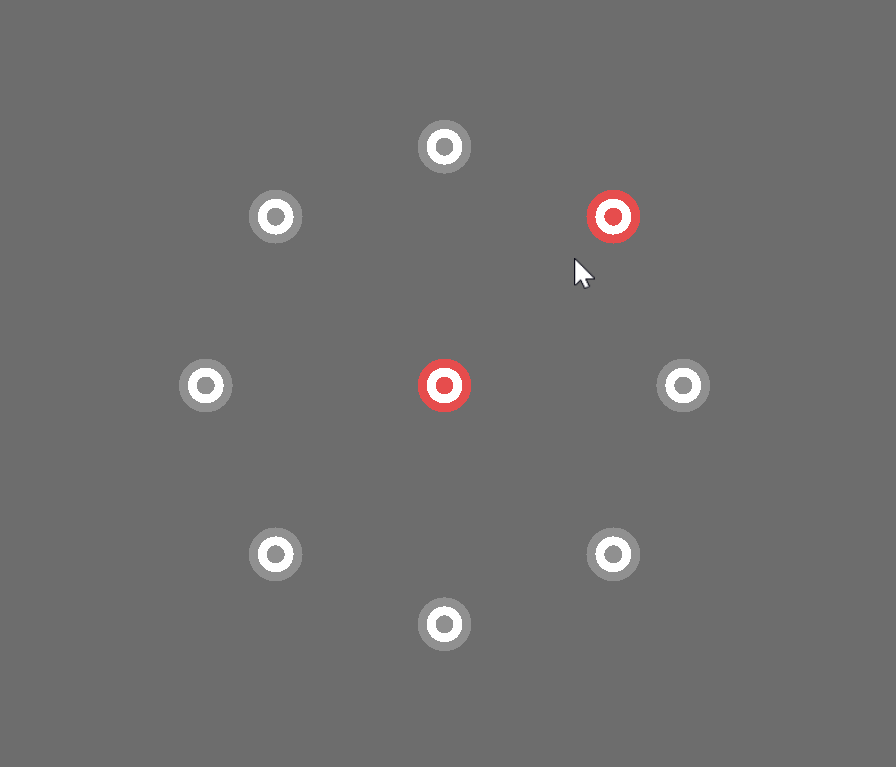
\includegraphics[width=55mm]{button.png}
 \caption{中央のボタンと,そのボタンからの距離と偏角が均等に配置される外側の8つのボタン}
 \label{button}
\end{figure}
\noindent

%%%%%%%%%%%%%%%%%%%%%%%%%

\subsubsection{カーソルの実装}
Windows OSが用意する標準のカーソルとは別に,Unity上で自作のカーソルを実装し,標準カーソルの座標の移動差分に調節可能なパラメータを乗算した差分を自作カーソルの座標に加えることで,カーソルの速さ調節を実現した.

本実験では,標準カーソルの速さをWindows OSの初期設定のものとし,その1.5倍,0.3倍の速さでカーソルの高速化と低速化を行った.この倍率は,予備実験時に最も快適に感じたものを採用している.

%%%%%%%%%%%%%%%%%%%%%%%%%

\subsection{被験者の選定}
本研究では,20代の男性2名,女性1名を対象に実験を行った.
より確実性の高い検証を行うためには,より幅広い年齢層やPC使用歴をもつ,より多くの被験者のデータを得る必要がある.

%%%%%%%%%%%%%%%%%%%%%%%%%

\subsection{被験者への説明}
画面を見せながら被験者に操作説明を行い,各手法の測定前に8セットのポインティングの練習を行わせた.被験者が機能に使い慣れた状態での動作性能を比較したいため,より確実性の高い検証のためには,時間の許す限りより多くの練習を行えるとよい.

速さと精度のバランスを保ったポインティングを被験者に行わせるために,全試行のうち7割はボタンの内側をポインティングできるように意識させ,かつ極力高速にポインティングを行うように指示をした.

%%%%%%%%%%%%%%%%%%%%%%%%%

\subsection{外れ値の除去}
得られたデータうち,軽微な位置修正では済まず,ポインティング時間が目立って長くなっているデータは外れ値として除外した.本実験では,箱ひげ図によってデータの分散具合を見たのちに,ポインティングに1秒以上かかったデータを除外した.

%%%%%%%%%%%%%%%%%%%%%%%%%

\subsection{ボタン外ポインティングのカウントと除外}
ポインティングの精度を調べるため,ボタンの外部をポインティングした回数(以下、エラー数とする)を測定した.

なお,分析の際には,ボタン外をポインティングしたデータは除去して考えた.


%%%%%%%%%%%%%%%%%%%%%%%%%%%%%%%%%%%%%%%%%%%%%%%%%%%%%%%%%%%%%%%%%%%%%%%%%%%%%%%%

\section{実験結果の分析}
\subsection{ポインティング精度の分析}
実験で得られたエラー数は,次の表\ref{hazurechi_cnt}の通りとなった.

サンプル数の少ない対応のあるデータを用いているため,Friedman検定を用いて,手法ごとのエラー数に有意差があるかを検定した.

検定は,漸近有意確率0.913で,エラー数に有意差があるとはいえない結果となった.つまりこれらのサンプルにおいて,提案する2手法は,従来手法と比べて精度が高いとも低いともいえないことがわかる.

\begin{table}[H]
 \centering
 \caption{各手法ごとのエラー数とその平均}
   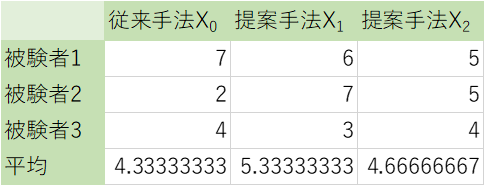
\includegraphics[width=65mm]{hazurechi_cnt.png}
 \label{hazurechi_cnt}
\end{table}
\noindent

%%%%%%%%%%%%%%%%%%%%%%%%%

\subsection{ポインティング時間の分析}
全被験者のポインティング時間を各手法ごとに箱ひげ図にまとめると,図~\ref{hakohige.png}の通りとなった(ボタン外部をポインティングしたデータと外れ値は除外している).

どの手法も平均と分散が近く,ポインティング時間が長くも短くもなっていない印象を受ける.また,正規分布に従いそうな,左右対称で中心にデータが多い分布を取っているため,目立った実験エラーはないものと考える.

\begin{figure}[H]
 \centering
   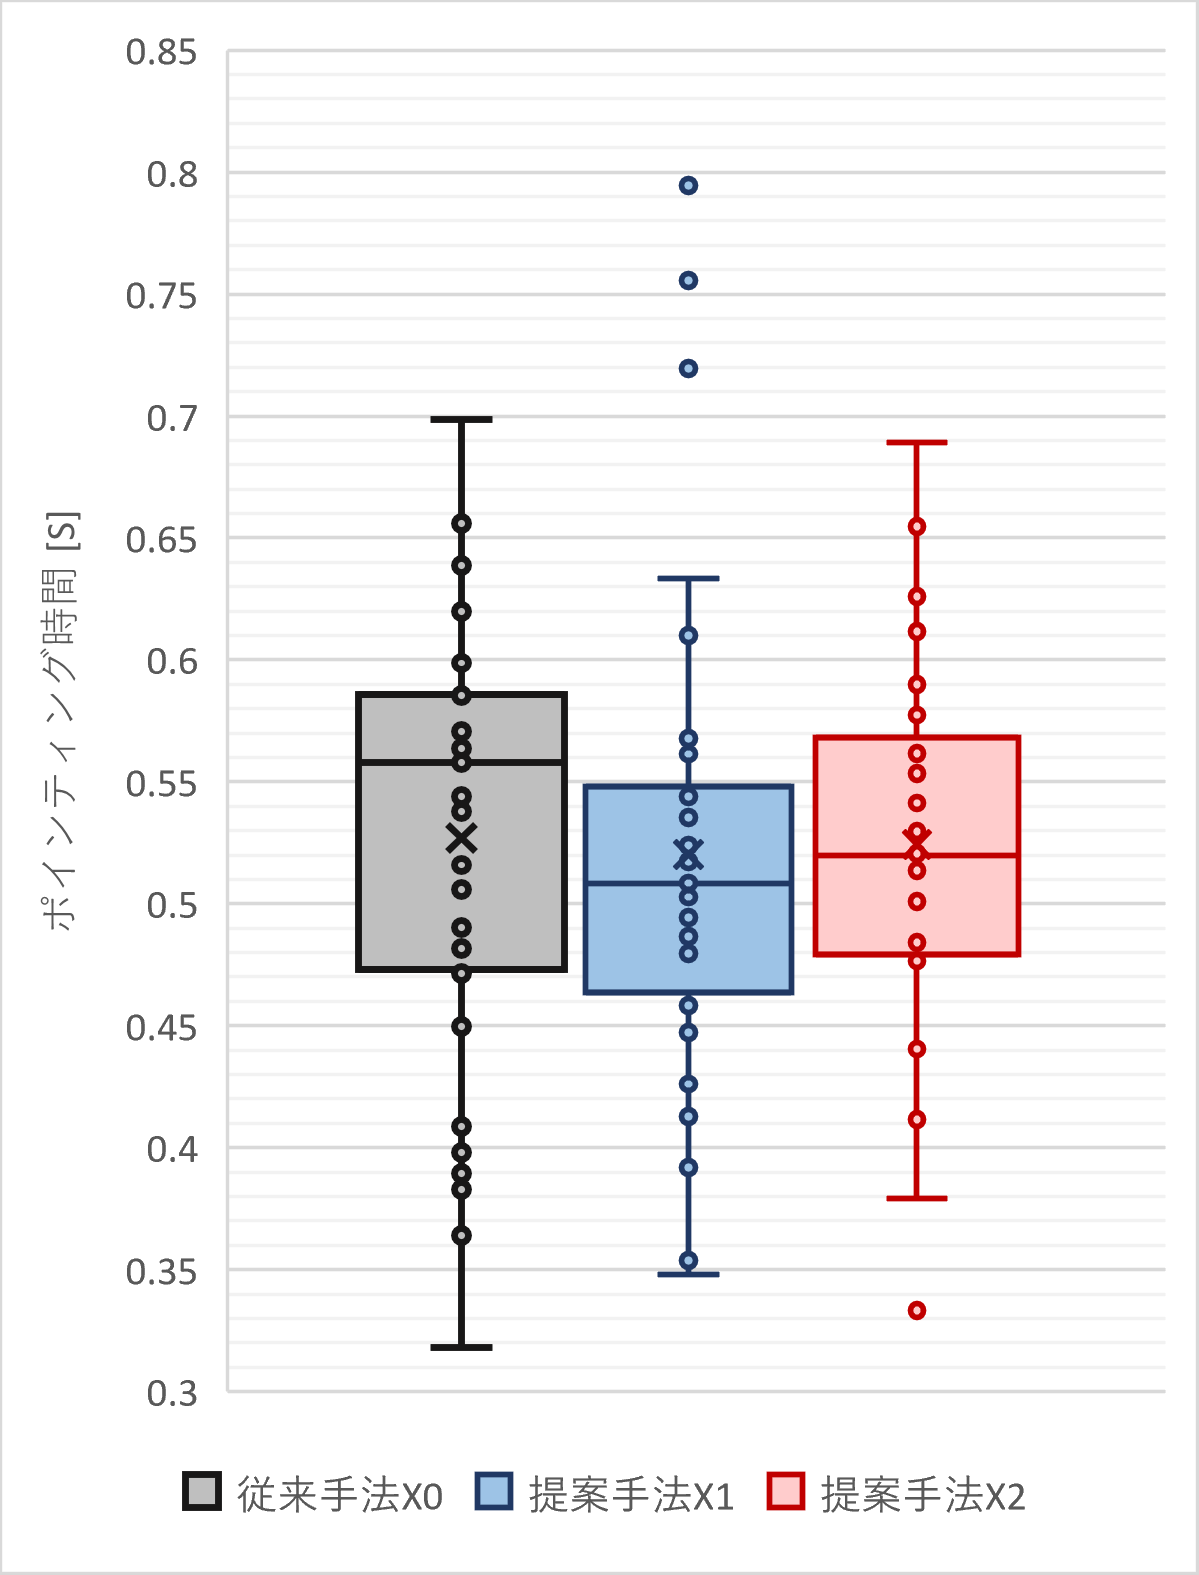
\includegraphics[width=65mm]{hakohige.png}
 \caption{各提案手法のポインティング時間の箱ひげ図}
 \label{hakohige}
\end{figure}
\noindent

手法ごとのポインティング時間に有意差があるか,Friedman検定を行って調査したところ,漸近有意確率0.552で,有意差があるとはいえない結果となった.つまりこれらのサンプルにおいて,提案する2手法は,従来手法と比べてポインティング時間が長いとも短いともいえないことがわかる.

%%%%%%%%%%%%%%%%%%%%%%%%%%%%%%%%%%%%%%%%%%%%%%%%%%%%%%%%%%%%%%%%%%%%%%%%%%%%%%%%

\section{議論}
20代の被験者3名を対象とした本実験では,ポインティングの時間と精度は,ともに有意に優れているとはいえない結果となった.しかし違う見方をすれば,被験者が不慣れな機能を使っているにも関わらず,「有意に劣っている(有意差があり,図表から劣っていることが明白である)」という結果にもなっていない.

つまり本実験の結果は,提案手法の有効性と習熟度不足が相殺されたために,従来手法との有意差があるとはいえないものになったのだと捉えられる.被験者からも「慣れによって快適になりそうだ」との意見が得られていたため,今回のデータだけでは,提案手法は否定しきれないものだと考える.

従って今後の課題として,提案手法の練習時間と時間・精度との関係を検証をすべきだと考える.

%%%%%%%%%%%%%%%%%%%%%%%%%%%%%%%%%%%%%%%%%%%%%%%%%%%%%%%%%%%%%%%%%%%%%%%%%%%%%%%%

\section{結論}
UI中のボタンの内外でカーソルの速さを調節する手法は,20代の被験者3名を対象とした短時間の練習を行う実験では,ポインティングの時間と精度が従来手法と比べて有意に優れているとはいえない結果となった.しかしながら,長時間の練習を行った後では,有意に優れている結果となることが少なからず期待できる.

%%%%%%%%%%%%%%%%%%%%%%%%%%%%%%%%%%%%%%%%%%%%%%%%%%%%%%%%%%%%%%%%%%%%%%%%%%%%%%%%

\begin{thebibliography}{99}

% F12 -> alert(document.lastModified); でサイトの更新日がわかる
\bibitem{report_1}
片岡凪(2020)
「仮説「ターゲットまでの距離が遠い場合,
ポインティングが完了するまでの時間は長い」の真偽の検証」,
\verb|<| \url{https://drive.google.com/file/d/18WbL6y6_yJ-OBGgYxApsGFiFZtw0Fcy1/view?usp=sharing} \verb|>|

\end{thebibliography}

\begin{comment}
メモ
\end{comment}

\end{multicols}

\end{document}
